\section{Syntax \& Aufbau eines \LaTeX -Dokuments}
 \begin{frame}
 	\frametitle{Inhalt}
 	\tableofcontents[%
 		currentsection, % causes all sections but the current to be shown in a semi-transparent way.
% % 		currentsubsection, % causes all subsections but the current subsection in the current section to ...
% % 		hideallsubsections, % causes all subsections to be hidden.
% 		hideothersubsections, % causes the subsections of sections other than the current one to be hidden.
% % 		part=, % part number causes the table of contents of part part number to be shown
% 		pausesections, % causes a \pause command to be issued before each section. This is useful if you
% 		pausesubsections, %  causes a \pause command to be issued before each subsection.
% % 		sections={ overlay specification },
 	]
 \end{frame}
\begin{frame}{Generelle Syntax}
	\begin{itemize}[<+->]
		\item alle Kommandos beginnen mit einem $\backslash$
		\item Kommentare mit einem \%
		\item Umgebungen beginnen mit $\backslash$begin\{ Umgebungsname\} und enden mit $\backslash$end\{Umgebungsname\}
	\end{itemize}
\end{frame}

\begin{frame}[fragile]{Beispiel Code}
	\lstsettex
	\begin{Code}
	\centering
		\begin{minipage}{0.9\textwidth}
	
		\lstinputlisting[linerange=1-19,title=\lstname]{./listings/demonstration.tex}
	
		\end{minipage}
	\end{Code}

\end{frame}
\begin{frame}[fragile]{Beispiel Code}
	\lstsettex
	\begin{Code}
	\centering
		\begin{minipage}{0.9\textwidth}
		\lstinputlisting[linerange=21-35,firstnumber=20,title=\lstname]{./listings/demonstration.tex}
		\end{minipage}
	\end{Code}

\end{frame}

\begin{frame}{Beispiel Ergebnis}
	\begin{figure}[tbph]
	\centering
	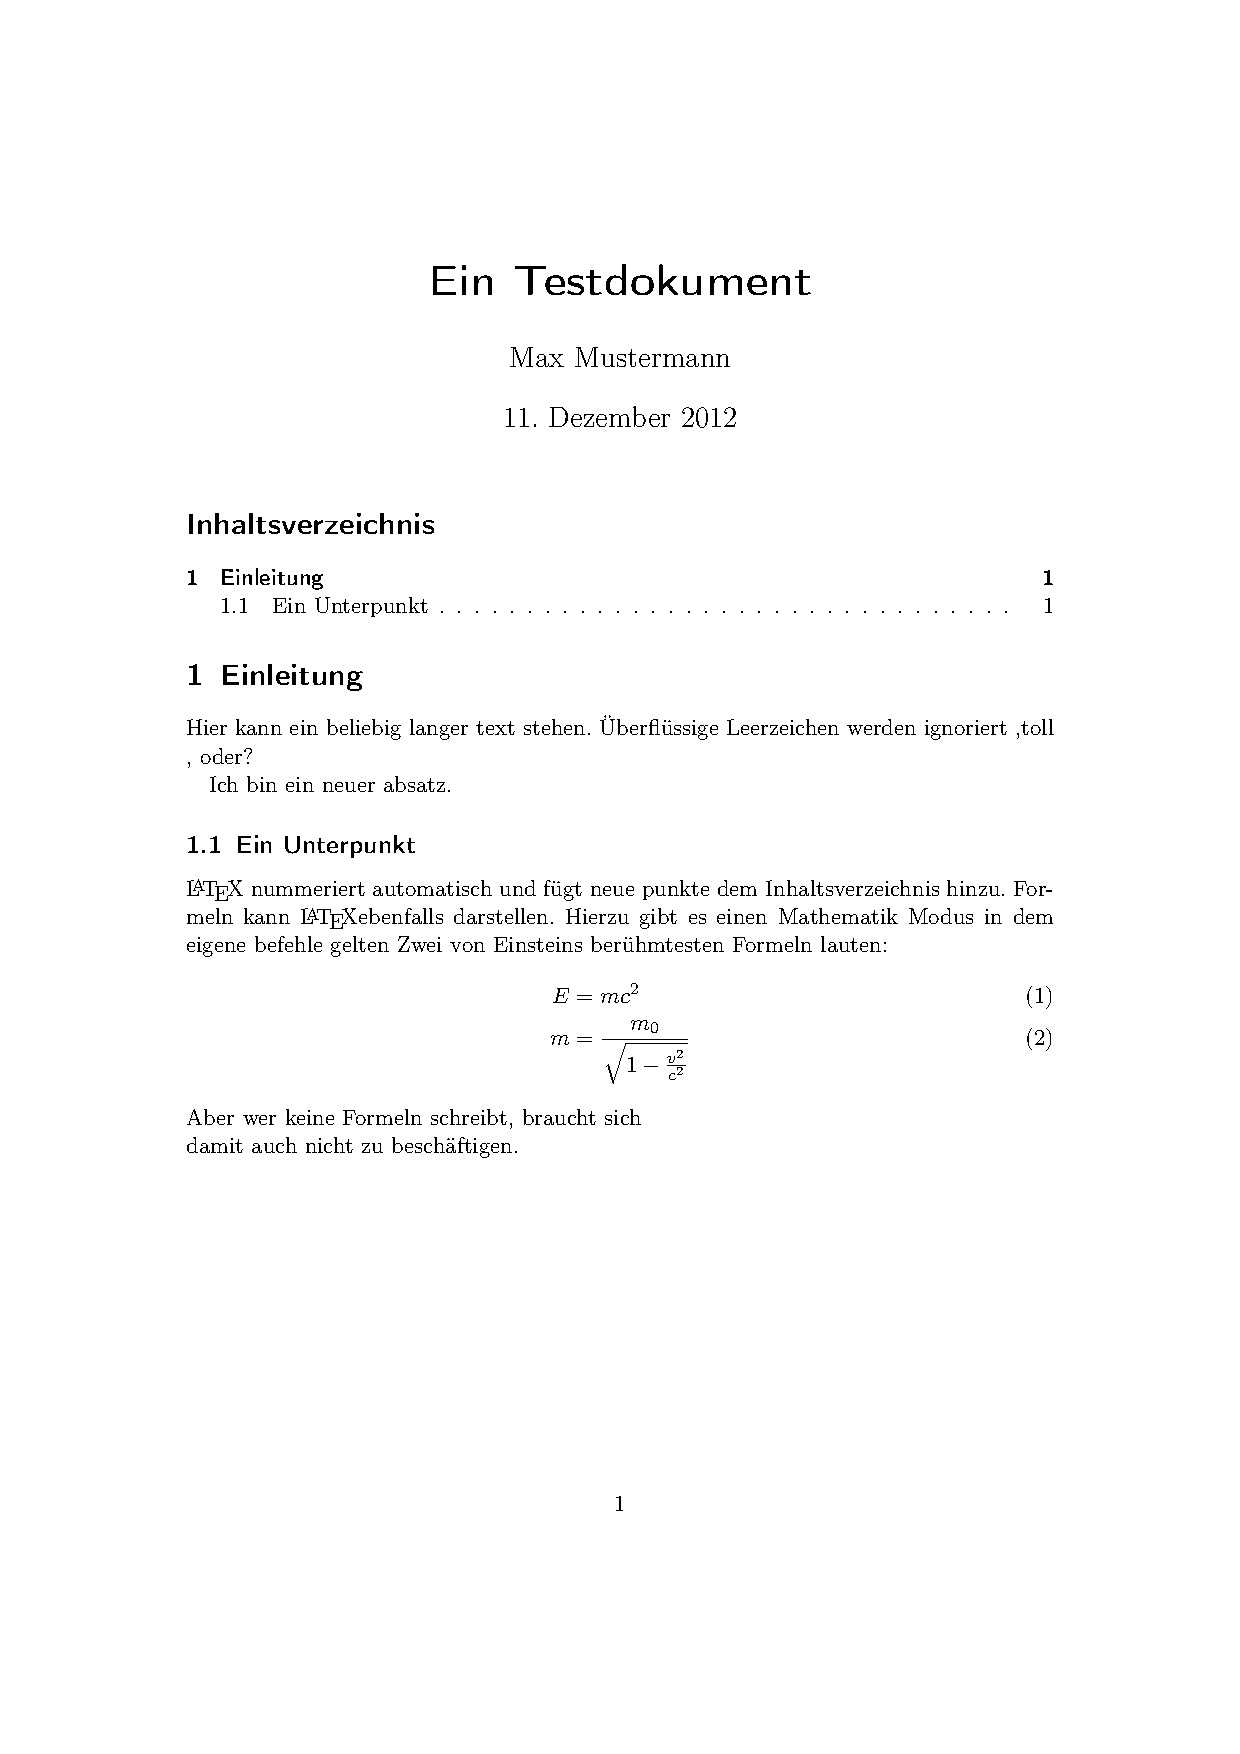
\includegraphics[height=\textheight]{./pictures/demonstration}
	\caption{Das PDF}
	\label{fig:demonstration}
	\end{figure}
\end{frame}

\begin{frame}{wichtige Befehle}
\lstsettex
	\begin{itemize}[<+->]
	\item \lstinputlisting[linerange=1-1]{./listings/commands.tex} $ \Rightarrow $ \textbf{fett}
	\item \lstinputlisting[linerange=2-2]{./listings/commands.tex} $ \Rightarrow $ \textit{kursiv}
	\item \lstinputlisting[linerange=3-3]{./listings/commands.tex} $ \Rightarrow $ \underline{unterstrichen}
	\item \lstinputlisting[linerange=4-4]{./listings/commands.tex} $ \Rightarrow $ \textbf{\textit{\underline{kombination}}}
	\end{itemize}
\end{frame}

\begin{frame}{Dokumentenklassen}
	\begin{itemize}[<+->]
		\item Briefe $ \Rightarrow $ letter,g-brief,scrlttr2
			\begin{itemize}[<+->]
				\item keine Gliederungsbefehle
			\end{itemize}
		\item Artikel $ \Rightarrow $ articel,scrartcl
			\begin{itemize}[<+->]
				\item section
				\item subsection
				\item subsubsection
			\end{itemize}
		\item Bericht $ \Rightarrow $ report, scrreprt
			\begin{itemize}[<+->]
				\item chapter
			\end{itemize}
		\item Bücher $ \Rightarrow $ book, scrbook
			\begin{itemize}[<+->]
				\item part
			\end{itemize}
		\item Präsentation $ \Rightarrow $ beamer
			\begin{itemize}[<+->]
				\item part
				\item section
				\item subsection
			\end{itemize}
	\end{itemize}
\end{frame}

\begin{frame}{Verzeichnisse}
\lstsettex
	\begin{itemize}[<+->]
	\item \lstinputlisting[linerange=5-5]{./listings/commands.tex}
	\item \lstinputlisting[linerange=6-6]{./listings/commands.tex}
	\item \lstinputlisting[linerange=7-7]{./listings/commands.tex}
	\item \lstinputlisting[linerange=8-8]{./listings/commands.tex}
	\end{itemize}
\end{frame}
\begin{frame}{Grafiken}
\lstsettex
\begin{Code}
\centering
\lstinputlisting[linerange=9-14,commentstyle=\small\color{sh_comment}\textit,
        keywordstyle=\small\color{sh_keyword}\bfseries,
        basicstyle=\small\ttfamily,
        stringstyle=\small\color{sh_string}\ttfamily]{./listings/commands.tex}
\end{Code}
\end{frame}
\begin{frame}{Grafiken}
\begin{figure}[tbph]
\centering

\includegraphics[width=0.7\linewidth]{./pictures/logo}
\caption[ich steh im Verzeichnis]{ich steh unter der Grafik}
\label{fig:logo-sm}
\end{figure}
\end{frame}
\begin{frame}{Tabellen}
\lstsettex
\begin{Code}
\centering
\lstinputlisting[linerange=15-25,commentstyle=\small\color{sh_comment}\textit,
        keywordstyle=\small\color{sh_keyword}\bfseries,
        basicstyle=\small\ttfamily,
        stringstyle=\small\color{sh_string}\ttfamily]{./listings/commands.tex}
\end{Code}
\end{frame}
\begin{frame}{Tabellen}
\begin{table}[tbph]
\centering
	\begin{tabular}{|*3{>{\centering\arraybackslash}m{0.2\textwidth}|}}
	\hline
	\textbf{kopf} & \textbf{kopf} & \textbf{kopf} \\ \hline
	inhalt & inhalt & inhalt \\ 
	inhalt & inhalt & inhalt \\ 
	\hline
	\end{tabular} 
	\caption[ich steh im Verzeichnis]{ich steh unter der Tabelle}
\end{table}
\end{frame}
\begin{frame}{Zitieren}
Voraussetzungen:\\
\pause
*.bib Datei\\
\pause
\lstsettex
\begin{Code}
\centering
\lstinputlisting[linerange=26-27,commentstyle=\small\color{sh_comment}\textit,
        keywordstyle=\small\color{sh_keyword}\bfseries,
        basicstyle=\small\ttfamily,
        stringstyle=\small\color{sh_string}\ttfamily]{./listings/commands.tex}
\end{Code}

\end{frame}
\begin{frame}{Bib-Datei Beispiel}
\lstsettex
\begin{Code}
\centering
\lstinputlisting[linerange=1-9,commentstyle=\small\color{sh_comment}\textit,
        keywordstyle=\small\color{sh_keyword}\bfseries,
        basicstyle=\small\ttfamily,
        stringstyle=\small\color{sh_string}\ttfamily]{./listings/bibliography.bib}
\end{Code}
\end{frame}
\begin{frame}{Auf BibTeX-Eintrag zugreifen}
\lstsettex
\begin{Code}
\centering
\lstinputlisting[linerange=28-29,commentstyle=\small\color{sh_comment}\textit,
        keywordstyle=\small\color{sh_keyword}\bfseries,
        basicstyle=\small\ttfamily,
        stringstyle=\small\color{sh_string}\ttfamily,caption={beliebige \TeX -Datei}]{./listings/commands.tex}
\end{Code}
\pause
ich zitiere hier \cite{braun:scala}\\
ich zitiere hier auch \footcite{braun:scala}
\end{frame}
\begin{frame}{Literaturverzeichnis}
\lstsettex
\begin{Code}
\centering
\lstinputlisting[linerange=30-30,commentstyle=\small\color{sh_comment}\textit,
        keywordstyle=\small\color{sh_keyword}\bfseries,
        basicstyle=\small\ttfamily,
        stringstyle=\small\color{sh_string}\ttfamily]{./listings/commands.tex}
\end{Code}
\printbibliography
\end{frame}